\documentclass[aspectratio=169, 12pt]{beamer}
 
\usepackage[utf8]{inputenc}
\usepackage{natbib, url}
\usepackage{enumerate, amsmath, amssymb, amsthm}
\usepackage{ragged2e} % make it justified
\justifying

% \usepackage{enumitem}
% \setlist{itemsep = 0pt, topsep = 1pt, leftmargin = 0.6mm}

\usepackage{hyperref}
\hypersetup{colorlinks, citecolor=blue, urlcolor=blue}
\usepackage{booktabs}
\usepackage{graphicx}


%\mode<presentation>{}
%\usepackage{beamerthemesplit} 

\setbeamertemplate{footline}[frame number]
%\setbeamertemplate{headline}{}
 
% slide 1
%Information to be included in the title page: % cohen was a prominent statistican and psychologist at NYU 
\title{Review of Jacob Cohen's The Earth is Round $(p < .05)$}

\author{Will Quinlan}
 
 
\begin{document}
 
\frame{\titlepage}

 % slide 2
\begin{frame}{An Introduction to Cohen's Paper}
  \begin{itemize}
  \item Scientific advancement has been hindered by null hypothesis testing (NHST)
  \item Researchers often misinterpret p-values restulting in mistakes in what can be concluded
  \item Critique the "ritualization" of NHST 
  \item Focus on real-world relevance
  \item Argues for better scientific practices
  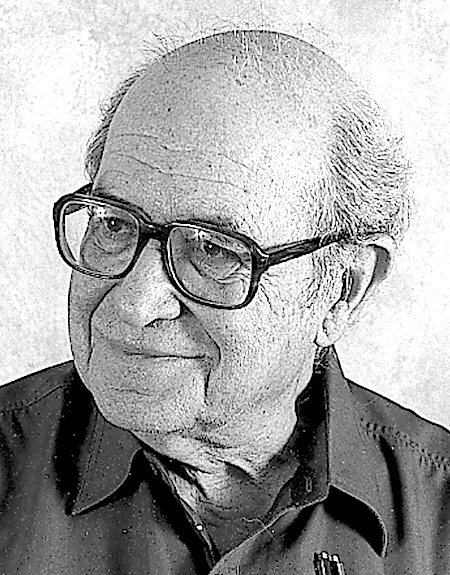
\includegraphics[width=0.15\textwidth]{./images/JacobCohen.png}
  \end{itemize}
\end{frame}

% slide 3
\begin{frame}{On Null Hypothesis Significance Testing}
  \begin{itemize}
  \item Definition: Method of statistical inference by which an experimental factor is tested against a hypothesis of no effect or no relationship based on a given observation
	\begin{itemize}
	\item In other words: Null vs Alternate
	\end{itemize}
  \item Decisions are determined by the signifiance threshold
  \item NHST dominates science
  \item If one presents a significant result of a known fact like "The Earth is round," nothing is gained
  \end{itemize}
\end{frame}

%Slide 4
\begin{frame}{A Ritualization of Reasoning $(p < .05)$}
  \begin{itemize}
  \item Cohen argues against the rigid reliance on p-values
  \item Standard p-value of .05
  \item Dichotomous reject-accept decision
  \item "The primary aim of a scientific experiment is not to precipitate decisions, but to make an appropriate adjustment in the degree to which one . . . believes the hypothesis . . . being
tested" - Bill Rozeboom (1960)
  \end{itemize}
\end{frame}

% Slide 5
\begin{frame}{Misinterpretation of p-values}
\begin{itemize} %[parsep=0pt, leftmargin=4mm, topsep=0pt, itemsep=0pt]
\item Consider a Scenario
   \begin{itemize}
   \item A scientist believes a certain disease does not exist 
   \item $H_0$: P = 0
   \item He draws a random sample of 30 cases and finds that 1 person has the disease
   \item $P_S$ = 1/30 = .033
   \end{itemize}
\item Does $H_0$ need testing with a chi-square? How about a Fischer exact test??
\item Cohen among many other scientists knows that academia would complain unless this result had a p-value attached to it
 \end{itemize}
\end{frame}

%Slide 6
\begin{frame}{So, what is wrong?}
  \begin{itemize}
  \item We think NHST tells us, "Given these data, what is the probability that $H_0$ is true?"
  \item What NHST actually tells us, "Given that $H_0$ is true, what is the probability of these (or more extreme) data?"
    before asking your question
  \item Academics have railed against NHST for many years before Cohen's paper
    \begin{itemize}
    \item "a potent but sterile intellectual rake who leaves in his merry path a long train of ravished maidens but no viable scientific offspring" - Meehl in 1967
    \item Joseph Berkson attacked NHST in 1938
    \item Lancelot Hogben's book-length critique appeared in 1957
    \end{itemize}
  \end{itemize}
\end{frame}


%Slide 7
\begin{frame}{The Permanent Illusion}
  \begin{itemize}
  \item Many believe the level of significance at which $H_0$ is rejected is the probability that it is correct 
  \item Syllogistic Reasoning according to Aristotle
	 \begin{itemize}
 	 \item If the null hypothesis is correct, then this datum (D) can not occur
	 \item D has, however, occurred
          \item Therefore, the null hypothesis is false.
 	 \end{itemize}
\item This is an example of a modus tollens syllogism, denying the antecedent by denying the consequent
	 \begin{itemize}
 	 \item If P, then Q 
	 \item Not Q (Q is false)
          \item Therefore, not P (P is false)
 	 \end{itemize}
  \end{itemize}
\end{frame}

%Slide 8
\begin{frame}{Probabilistic Syllogism}
  \begin{itemize}
  \item What if the syllogism is probabilistic?
    \begin{itemize}
    \item If the null hypothesis is correct, then these data are highly unlikely
    \item These data have occurred
    \item Therefore, the null hypothesis is highly unlikely
    \end{itemize}
  \item This makes what was a valid modus tollens syllogism formally invalid %syllogims must deal with true-false to be formally valid
	 \begin{itemize}
 	 \item If P, then Q is likely
	 \item Not Q
          \item Therefore, P is unlikely
 	 \end{itemize}
  \end{itemize}
\end{frame}

%Slide 9
\begin{frame}{Examples of Syllogisms}
  \begin{itemize}
  \item Some Examples:
    \begin{itemize}
    \item If a person is a Martian, then he is not a member of Congress
    \item This person is a member of Congress
    \item Therefore, he is not a Martian
    \end{itemize}
  \item How about this one?
    \begin{itemize}
    \item If a person is an American, then he is not a member of Congress  %the major premise is false here, so this syllogism is not sensible, but it is still formally correct
    \item This person is a member of Congress
    \item Therefore, he is not an American
    \end{itemize}
  \end{itemize}
\end{frame}

%Slide 10
\begin{frame}{Examples of Syllogisms cont.}
  \begin{itemize}
  \item What about now?
    \begin{itemize}
    \item If a person is an American, then he is probably not a member of Congress %probabilistic here, syllogism is formally incorrect which leads to a nonsensible conclusion
    \item This person is a member of Congress
    \item Therefore, he is probably not an American
    \end{itemize}
  \item This last one?
    \begin{itemize}
    \item If $H_0$ is true, then this result (statistical significance) would probably not occur %this if formally the exact same as the previous example, and this is also formally invalid
    \item This result has occurred
    \item Therefore, $H_0$ is probably not true
    \end{itemize}
  \end{itemize}
\end{frame}

%Slide 11
\begin{frame}{P(D$|$$H_0$) \neq P($H_0$$|$D)}
  \begin{itemize}
  \item When testing $H_0$, one is finding the probability data (D) could have arisen if $H_0$ were true, P(D$|$$H_0$)
  \item If this probability is small, one can conclude that $H_0$ is true and D is unlikely
  \item What about the reverse probability P($H_0$$|$D)?
    \begin{itemize}
    \item When rejecting $H_0$, one wants to conclude $H_0$ is unlikely
    \item This probability is only available through Bayes theorem where we need to know P($H_0$)
    \item Bayesian statisticians use a prior probability or distribution of probabilities to deal with this problem, but does it hold up?
    \end{itemize}
  \end{itemize}
\end{frame}

%Slide 12
\begin{frame}{A Look at Psychiatric Diagnoses}
  \begin{itemize}
  \item Incidence of schizophrenia in adults is 2\%\
  \item A proposed screening test is estimated to have 95\% accuracy (P(normality$|$$H_0$) \(\approx\) 0.95)
  \item The screening test is supposed to have 97\% accuracy in declaring normality (P(schizophrenia$|$$H_1$) \(>\) 0.97)
  \item Thus, we have a test that is highly sensitive and highly specific
    \begin{itemize}
    \item $H_0$ = The case is normal
    \item $H_1$ = The case is schizophrenic
    \item D = The test result (the data) is positive for schizophrenia
    \end{itemize}
  \end{itemize}
\end{frame}

%Slide 13
\begin{frame}{A Look at Psychiatric Diagnoses cont.}
  \begin{itemize}
  \item P(D$|$$H_0$) \(<\) .05 seems like what we want, but it is not
  \item We want P($H_0$$|$D) which equals .60, not the .05 we may have believed
\[
P(H_0 | D) = \frac{P(H_0) \cdot P(\text{test wrong} | H_0)}{P(H_0) \cdot P(\text{test wrong} | H_0) + P(H_1) \cdot P(\text{test correct} | H_1)}
\]
\item Schizophrenic
\begin{tabular}{ccccc}
  \toprule
 Result &   Normal & Schiz & Total \\
  \midrule
 Negative Test (Normal)  &  949     &   1           &  950        \\
 Positive Test (Schiz)  &  30      &    20          &  50        \\
 Total    &  979      & 21          & 1,000         \\
  \bottomrule
%Cohen says this is a common phenomena in textbooks and even among academics. This inverse probability error is all too common. This was an error made by 68 of 70 academics in a study performed by Oakes in 1986
\end{tabular}
  \end{itemize}
\end{frame}

%Slide 12
\begin{frame}{Replication}
  \begin{itemize}
  \item The error previously demonstrated can also be applied to replication of tests
  \item If there was a successful rejection of $H_0$ many believe replications will also result in the rejection of $H_0$
  \item Many believe that a p of .99 means 99\% of the time a result will replicate
  \item Typical level of power for medium effect sizes of .50
    \begin{itemize}
    \item The chances are in three replications only one in eight would result in significant results
    \end{itemize}
  \end{itemize}
\end{frame}

%Slide 13
\begin{frame}{More Syllogisms}
  \begin{itemize}
  \item We have just seen many failures in logic by researchers such as if $H_0$ is rejected, then the theorey is established. Invalid syllogism and example below: 
    \begin{itemize}
    \item If it rains (A), then the ground will be wet (B).
    \item The ground is wet (B).
    \item Therefore, it rained (A).
    \end{itemize}
  \item However, even if a valid modus tollens syllogism in used, misinterpretations are still made
    \begin{itemize}
   \item When $H_0$ is rejected, it can be because of a variety of auxillary theories, and not what precipitated the research
   \item Although it is convenient, accept-reject decisions; although convenient, are not how science is done
    \end{itemize}
  \end{itemize}
\end{frame}

%Slide 14
\begin{frame}{The Nil Hypothesis}
  \begin{itemize}
  \item Some propositions consider what is occuring within a population (i.e. the proportion of males in this population is .75)
  \item Cohen refers to the $H_0$ when the effect size = 0 as the nil hypothesis
  \item Effecet size is effectively the practical significance of a test
  \item However, universally $H_0$ is taken to mean nil (zero), Ex:
    \begin{itemize}
    \item $H_0$ is the proportion of males in a population if .50
    \item $H_0$ is the raters reliability is 0
    \end{itemize}
  \item These are cases when $H_0$ is almost universally rejected
  \item Tukey wrote, "It is foolish to ask 'Are the effects of A and B different?' They are always different—for some decimal place"
  \end{itemize}
\end{frame}

%Slide 15
\begin{frame}{The Illusion of Proof}
  \begin{itemize}
  \item Virtual participants: put questions into the Q/A window in WebEx
  \item In-person participants: walk to a microphone and wait to be called upon
    before asking your question
  \item Lunch on your own (Student Union food court right next door)x
  \item Coffee/cookies available during the poster session (11:30--13:30)
  \item Training workshops:
    \begin{itemize}
    \item Each workshop has its own (webex meeting) room
    \item Virtual participants please mute yourself in each session.
    \end{itemize}
  \end{itemize}
\end{frame}

%Slide 16
\begin{frame}{The Illusion of Proof}
  \begin{itemize}
  \item Virtual participants: put questions into the Q/A window in WebEx
  \item In-person participants: walk to a microphone and wait to be called upon
    before asking your question
  \item Lunch on your own (Student Union food court right next door)x
  \item Coffee/cookies available during the poster session (11:30--13:30)
  \item Training workshops:
    \begin{itemize}
    \item Each workshop has its own (webex meeting) room
    \item Virtual participants please mute yourself in each session.
    \end{itemize}
  \end{itemize}
\end{frame}

%Slide 17
\begin{frame}{The Illusion of Proof}
  \begin{itemize}
  \item Virtual participants: put questions into the Q/A window in WebEx
  \item In-person participants: walk to a microphone and wait to be called upon
    before asking your question
  \item Lunch on your own (Student Union food court right next door)x
  \item Coffee/cookies available during the poster session (11:30--13:30)
  \item Training workshops:
    \begin{itemize}
    \item Each workshop has its own (webex meeting) room
    \item Virtual participants please mute yourself in each session.
    \end{itemize}
  \end{itemize}
\end{frame}

%Slide 18
\begin{frame}{The Illusion of Proof}
  \begin{itemize}
  \item Virtual participants: put questions into the Q/A window in WebEx
  \item In-person participants: walk to a microphone and wait to be called upon
    before asking your question
  \item Lunch on your own (Student Union food court right next door)x
  \item Coffee/cookies available during the poster session (11:30--13:30)
  \item Training workshops:
    \begin{itemize}
    \item Each workshop has its own (webex meeting) room
    \item Virtual participants please mute yourself in each session.
    \end{itemize}
  \end{itemize}
\end{frame}

%Slide 19
\begin{frame}{The Illusion of Proof}
  \begin{itemize}
  \item Virtual participants: put questions into the Q/A window in WebEx
  \item In-person participants: walk to a microphone and wait to be called upon
    before asking your question
  \item Lunch on your own (Student Union food court right next door)x
  \item Coffee/cookies available during the poster session (11:30--13:30)
  \item Training workshops:
    \begin{itemize}
    \item Each workshop has its own (webex meeting) room
    \item Virtual participants please mute yourself in each session.
    \end{itemize}
  \end{itemize}
\end{frame}

%Slide 20
\begin{frame}{The Illusion of Proof}
  \begin{itemize}
  \item Virtual participants: put questions into the Q/A window in WebEx
  \item In-person participants: walk to a microphone and wait to be called upon
    before asking your question
  \item Lunch on your own (Student Union food court right next door)x
  \item Coffee/cookies available during the poster session (11:30--13:30)
  \item Training workshops:
    \begin{itemize}
    \item Each workshop has its own (webex meeting) room
    \item Virtual participants please mute yourself in each session.
    \end{itemize}
  \end{itemize}
\end{frame}
%Slide 21
\begin{frame}{The Illusion of Proof}
  \begin{itemize}
  \item Virtual participants: put questions into the Q/A window in WebEx
  \item In-person participants: walk to a microphone and wait to be called upon
    before asking your question
  \item Lunch on your own (Student Union food court right next door)x
  \item Coffee/cookies available during the poster session (11:30--13:30)
  \item Training workshops:
    \begin{itemize}
    \item Each workshop has its own (webex meeting) room
    \item Virtual participants please mute yourself in each session.
    \end{itemize}
  \end{itemize}
\end{frame}


\end{document}
